%%%%%%%%%%%%%%%%%%%%%%%%%%%%%%%%%%%%%%%%%%%%%%%%%%%%%%%%%%%%%%%%%%%%%%%%%%%%%%%%%%
\begin{frame}[fragile]\frametitle{}
\begin{center}
{\Large Introduction}
\end{center}
\end{frame}


%%%%%%%%%%%%%%%%%%%%%%%%%%%%%%%%%%%%%%%%%%%%%%%%%%%%%%%%%%%
\begin{frame}[fragile]\frametitle{Calling the Call Center}
	\begin{itemize}
	\item Calling to an IVR (Integrated Voice Response)
	\item A pre-recorded menu selection.
	\item ``Please press 1 for Account Details, Please press 2 for \ldots''
	\item Till it comes to your option. 
	\item Else, you are given access to a person to talk to.
	\end{itemize}

Boring? Annoying? But still heavily used \ldots, Why?

\begin{center}
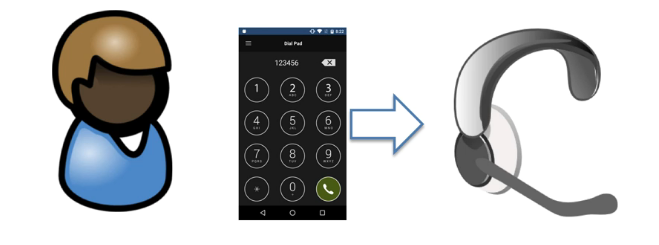
\includegraphics[width=0.5\linewidth,keepaspectratio]{nlp10}

\tiny{(Ref: Deep Learning and NLP A-Z - Kirill Eremenko)}
\end{center}
Instead, how about typing/saying your query directly and getting the answer right away?

\end{frame}

%%%%%%%%%%%%%%%%%%%%%%%%%%%%%%%%%%%%%%%%%%%%%%%%%%%%%%%%%%%
\begin{frame}[fragile]\frametitle{Solution}
Chatbots!!!

	\begin{itemize}
	\item Which problem of IVR it is solving?
	\item Advantages?
	\item Disadvantages?
	\item Gaining popularity \ldots
	\item Many platforms
	\item Companies in Pune?
	\end{itemize}


\end{frame}

%%%%%%%%%%%%%%%%%%%%%%%%%%%%%%%%%%%%%%%%%%%%%%%%%%%%%%%%%%%
\begin{frame}[fragile]\frametitle{Crystal Ball}

\begin{itemize}
\item 85\% Of customer interactions will be managed without a human by 2020 – Gartner prediction

\item ``The global chatbot market is expected to reach \$1.23 billion by 2025'' - Business Insider
\end{itemize}

\end{frame}

%%%%%%%%%%%%%%%%%%%%%%%%%%%%%%%%%%%%%%%%%%%%%%%%%%%%%%%%%%%
\begin{frame}[fragile]\frametitle{Sample Application}

SnapTravel has processed \$1 million in hotel bookings inside Messenger.


\begin{center}
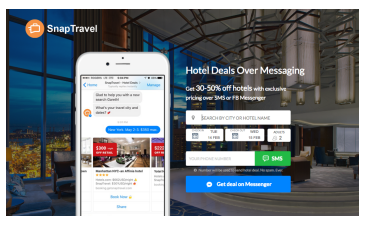
\includegraphics[width=\linewidth,keepaspectratio]{chatbot28}
\end{center}

{\tiny (Ref: Innovation in Health - Ritesh Ptael, et al)}


\end{frame}



%%%%%%%%%%%%%%%%%%%%%%%%%%%%%%%%%%%%%%%%%%%%%%%%%%%%%%%%%%%
\begin{frame}[fragile]\frametitle{So, What is a Chatbot?}

``Chatbots are a form of human-computer dialog system which operates 
through natural language via text or speech''- Deryugina, 2010; Sansonnet et al., 2006.

\begin{center}
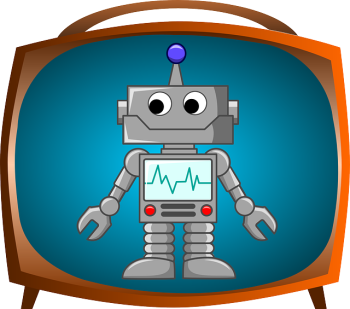
\includegraphics[width=0.4\linewidth,keepaspectratio]{chatbot37}

{\tiny (Ref: Rasa - mdd01 course on github )}

\end{center}

\end{frame}


%%%%%%%%%%%%%%%%%%%%%%%%%%%%%%%%%%%%%%%%%%%%%%%%%%%%%%%%%%%
\begin{frame}[fragile]\frametitle{Anatomy of a Chatbot}

\begin{center}
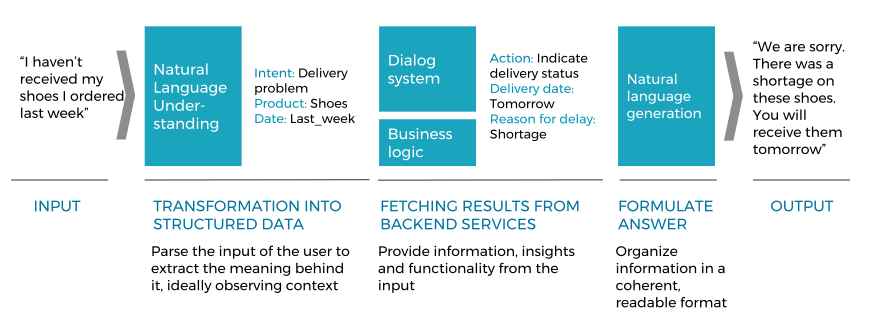
\includegraphics[width=\linewidth,keepaspectratio]{chatbot52}

{\tiny (Ref: Chatbots and AI - botfuel )}

\end{center}

\end{frame}

% %%%%%%%%%%%%%%%%%%%%%%%%%%%%%%%%%%%%%%%%%%%%%%%%%%%%%%%%%%%
% \begin{frame}[fragile]\frametitle{Chatbot: Examples}

% \begin{itemize}
% \item Cornell Bot https://microsoft.github.io/techcasestudies/bot\%20framework/2017/06/15/WeillCornell.html
% \item  Erica Part 1https://www.forbes.com/sites/quora/2016/10/28/meet-erica-bank-of-americas-new-voice-ai-banking-system/\#28ab9b6d50db
% \item Erica Part 2https://www.bizjournals.com/charlotte/news/2018/05/21/bank-of-america-rolls-out-ai-assistant-erica-to.html
% \item Tia part 1 https://rasa.com/solutions/healthcare/ Tia part 2 https://www.asktia.com/app/
% \item Cora https://www.ibm.com/industries/banking-financial-markets/front-office/chatbots-banking
% \item Raiffeisen https://rasa.com/customers/raiffeisen
% \item Eno https://www.forbes.com/sites/capitalone/2017/10/19/becoming-a-bot-ai-design-and-the-incomparable-eno/\#681ccfffebc2
% \item Helvetia https://rasa.com/customers/helvetia-claims
% \item SmartCom https://rasa.com/customers/telecom-upgrades
% \item Travel Bot https://rasa.com/customers/travel-assistant
% \end{itemize}

% {\tiny (Ref: Rasa - mdd01 course on github )}
% \end{frame}


%%%%%%%%%%%%%%%%%%%%%%%%%%%%%%%%%%%%%%%%%%%%%%%%%%%%%%%%%%%
 \begin{frame}[fragile]\frametitle{Why so many chatbot startups?}
\begin{itemize}
\item VCs appear excited with this new tool, more services, more opportunities, new battlegrounds for the big players (likely leading to acquisitions). 
\item So even without real technological breakthroughs, there is at least some money to be made investing in bot startups.
\item But the real issue is : Truly `conversational' software is a difficult problem to solve.
\end{itemize}

{\tiny (Ref: We don't know how to build conversational software yet (Alan Nichol Apr 2016))}
\end{frame}

%%%%%%%%%%%%%%%%%%%%%%%%%%%%%%%%%%%%%%%%%%%%%%%%%%%%%%%%%%%
 \begin{frame}[fragile]\frametitle{How difficult?}

\begin{center}
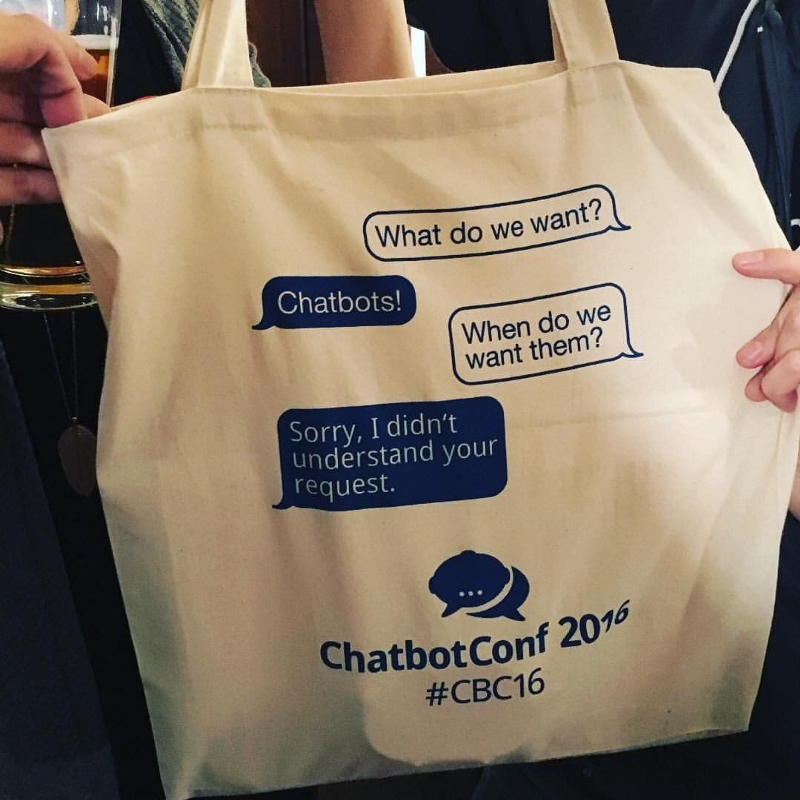
\includegraphics[width=0.5\linewidth,keepaspectratio]{chatbot21}

\end{center}

So what tools do developers need to do better than this?


{\tiny (Ref: A New Approach to Conversational Software - Alan Nichol)}
\end{frame}

%%%%%%%%%%%%%%%%%%%%%%%%%%%%%%%%%%%%%%%%%%%%%%%%%%%%%%%%%%%
\begin{frame}[fragile]\frametitle{NLU is AI}

Understanding Natural Language is Hallmark of Artificial Intelligence!!

\begin{center}
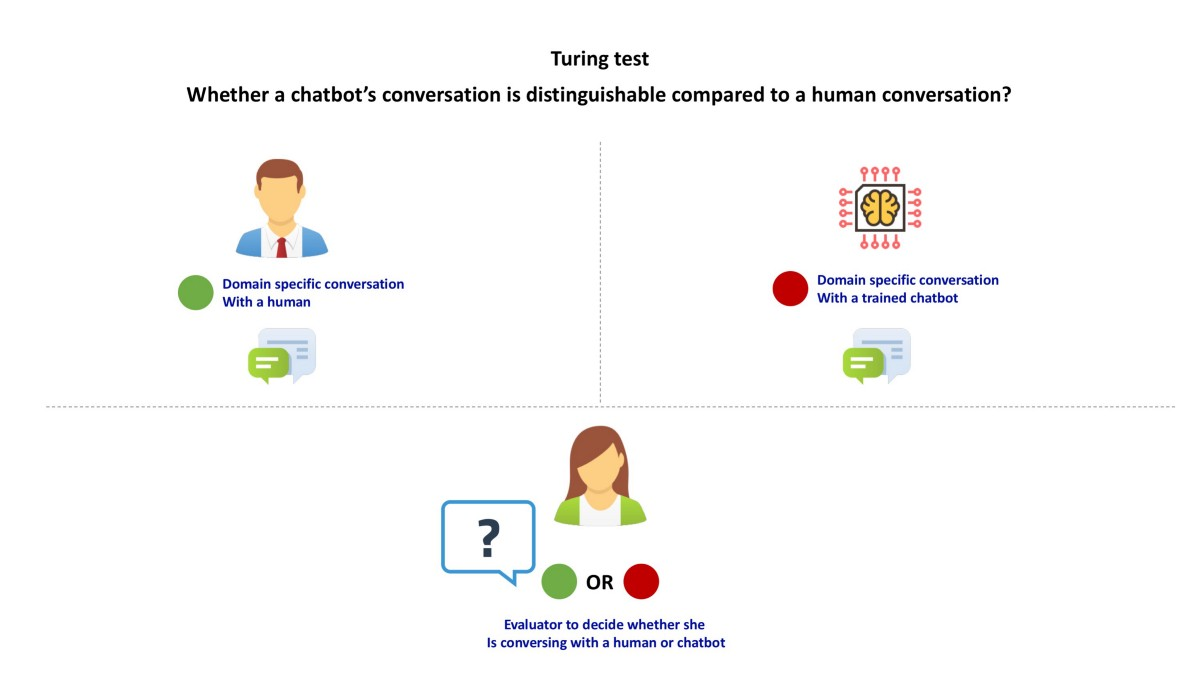
\includegraphics[width=\linewidth,keepaspectratio]{chatbot29}
\end{center}

{\tiny (Ref: Conversational AI: Understanding the Basics and Building a Chatbot in Rasa module - Manikandan Jeeva)}
\end{frame}

%%%%%%%%%%%%%%%%%%%%%%%%%%%%%%%%%%%%%%%%%%%%%%%%%%%%%%%%%%%
\begin{frame}[fragile]\frametitle{NLU is AI}

\begin{center}
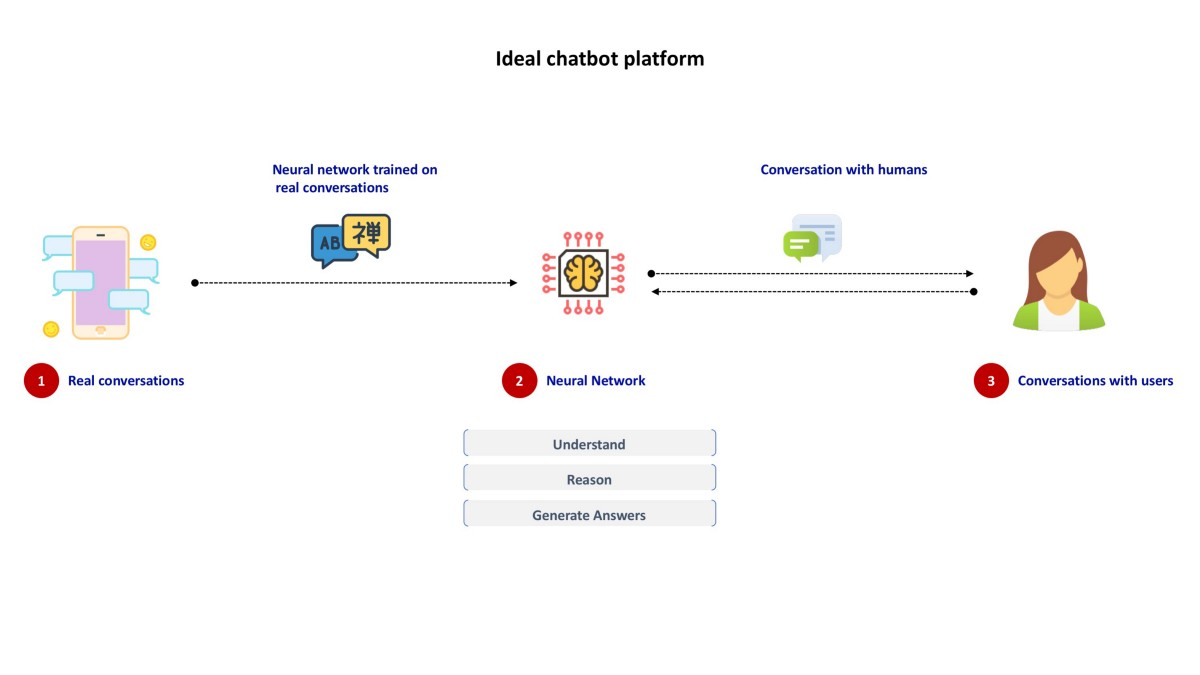
\includegraphics[width=\linewidth,keepaspectratio]{chatbot30}
\end{center}

But the current bots are not this generic.

{\tiny (Ref: Conversational AI: Understanding the Basics and Building a Chatbot in Rasa module - Manikandan Jeeva)}
\end{frame}


%%%%%%%%%%%%%%%%%%%%%%%%%%%%%%%%%%%%%%%%%%%%%%%%%%%%%%%%%%%
\begin{frame}[fragile]\frametitle{Types of Chatbots}
\begin{itemize}
\item Command \& response: Stateless bots are essentially a command line app over HTTP
\item Hard-coded conversation flows: navigate a flow chart defined. http://superscriptjs.com/ allows that. Evi is an intelligent bot built with ``knowledge base'' technology.
\item Fuzzy/continuous/fluid state: that's the goal. Human conversations don't follow a template
\end{itemize}

{\tiny (Ref: We don't know how to build conversational software yet (Alan Nichol Apr 2016))}
\end{frame}

%%%%%%%%%%%%%%%%%%%%%%%%%%%%%%%%%%%%%%%%%%%%%%%%%%%%%%%%%%%
\begin{frame}[fragile]\frametitle{Classification of Chatbots}
    \begin{columns}
    \begin{column}[t]{0.5\linewidth}
	
\begin{center}
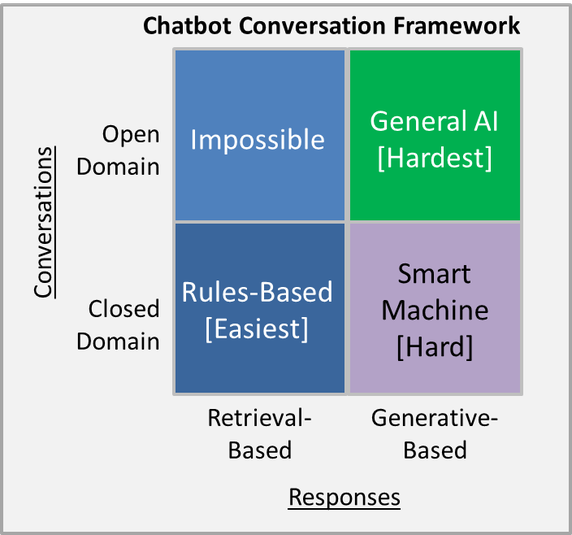
\includegraphics[width=\linewidth,keepaspectratio]{chatbot24}
\end{center}
    \end{column}
    \begin{column}[t]{0.5\linewidth}

\begin{itemize}
\item Retrieval-based models (easier) use a repository of predefined responses and some kind of heuristic to pick an appropriate response based on the input and context. 
\item Generative models (harder) are based on Machine Translation techniques, but instead of translating from one language to another, we ``translate'' from an input to an output (response).
\end{itemize}
    \end{column}
    \end{columns}

% {\tiny (Ref: https://www.quora.com/How-can-I-build-an-intelligent-chat-bot)}
\end{frame}



% %%%%%%%%%%%%%%%%%%%%%%%%%%%%%%%%%%%%%%%%%%%%%%%%%%%%%%%%%%%
% \begin{frame}[fragile]\frametitle{Retrieval based chatbot}

% The way it works:

% \begin{itemize}
% \item You supply FAQs in the form of csv (comma separated file) having Question-Answer-Class in each row (e.g. "What is GST rate for Toothpaste?,12,rate")
% \item Questions are vectorized and kept ready for matching, along with the classifier model [X=vector(question), y=class]
% \item Once user query comes, its 'class' is predicted using the classifier model and within the class, vectorized query is matched against existing vectorized questions.
% \item Whichever is most similar, it's answer is presented to the user.
% \end{itemize}


% So,
% \begin{itemize}
% \item Similarity based
% \item Atomic
% \item Can handle simple questions and respond with pre-built responses based on rule-based conversation processing. 
% \item For instance, if user says X, respond with Y; if user says Z, call a REST API, and so forth.
% \end{itemize}

% \end{frame}

% %%%%%%%%%%%%%%%%%%%%%%%%%%%%%%%%%%%%%%%%%%%%%%%%%%%%%%%%%%%
% \begin{frame}[fragile]\frametitle{Dialog flow based chatbot}

% \begin{itemize}
% \item Decision Tree traversal
% \item Slot filling
% \item Knows the context (previous chat history as well as sub domain)
% \item Five levels of AI assistants: From notification assistants to autonomous organizations
% \end{itemize}

% \end{frame}




% % %%%%%%%%%%%%%%%%%%%%%%%%%%%%%%%%%%%%%%%%%%%%%%%%%%%%%%%%%%%
% % \begin{frame}[fragile]\frametitle{AI Levels}
% % Five levels of AI assistants: From notification assistants to autonomous organizations

% % \begin{center}
% % 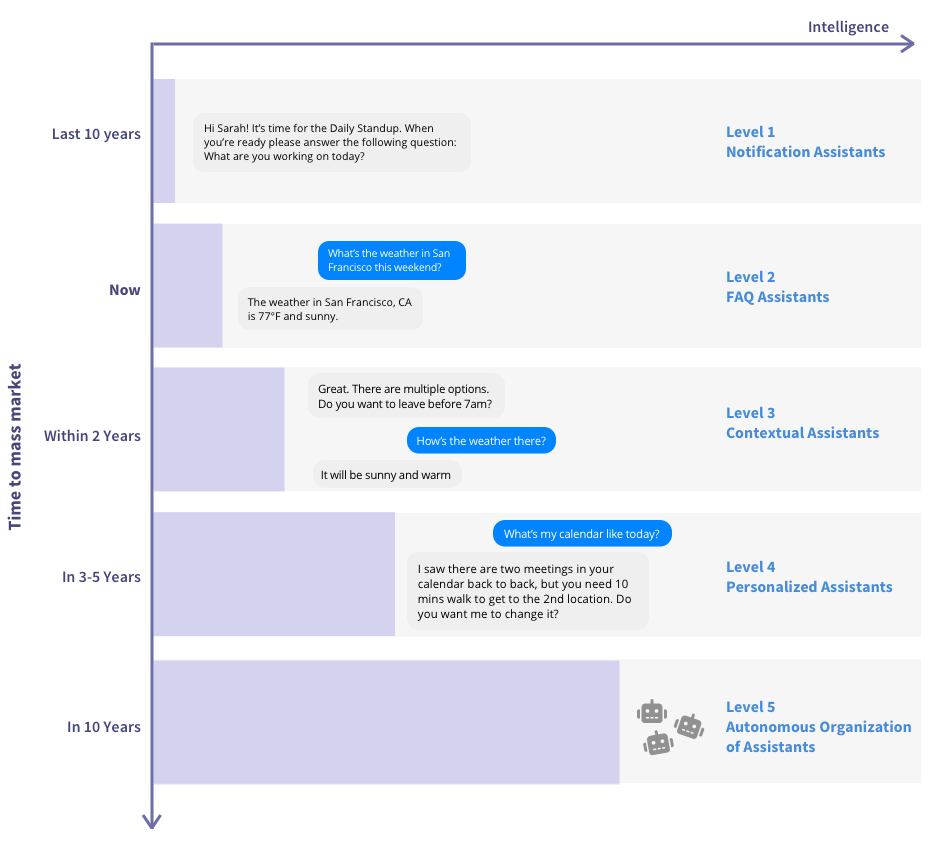
\includegraphics[width=0.6\linewidth]{chatbot1}
% % \end{center}

% % % {\tiny (Ref: The next generation of AI assistants in enterprise -  Alan Nichol)}
% % \end{frame}

% %%%%%%%%%%%%%%%%%%%%%%%%%%%%%%%%%%%%%%%%%%%%%%%%%%%%%%%%%%%
% \begin{frame}[fragile]\frametitle{Level 1 : Notification Assistants}
% \begin{itemize}
% \item The chatbot is essentially a traditional notification assistant; it can answer a question with a pre-built response. 
% \item It can send you notifications about certain events or reminders about things in which you've explicitly expressed interest. 
% \item For instance, a level 1 travel bot can provide a link for you to book travel.
% \end{itemize}

% \begin{center}
% 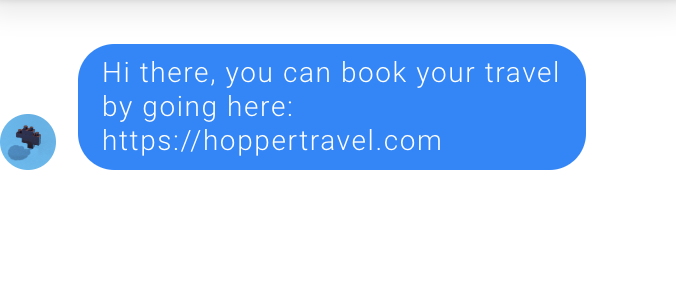
\includegraphics[width=0.6\linewidth,keepaspectratio]{chatbot13}
% \end{center}

% % {\tiny (Ref: The next generation of AI assistants in enterprise -  Alan Nichol)}
% \end{frame}

% %%%%%%%%%%%%%%%%%%%%%%%%%%%%%%%%%%%%%%%%%%%%%%%%%%%%%%%%%%%
% \begin{frame}[fragile]\frametitle{Level 2 : FAQ Assistants}
% \begin{itemize}
% \item The chatbot can answer FAQs 
% \item but is also capable of handling a simple follow up.
% \end{itemize}

% \begin{center}
% 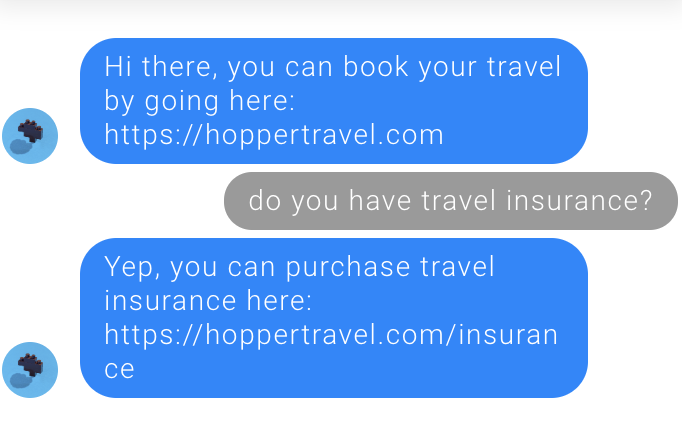
\includegraphics[width=0.6\linewidth,keepaspectratio]{chatbot14}
% \end{center}

% % {\tiny (Ref: The next generation of AI assistants in enterprise -  Alan Nichol)}
% \end{frame}

% %%%%%%%%%%%%%%%%%%%%%%%%%%%%%%%%%%%%%%%%%%%%%%%%%%%%%%%%%%%
% \begin{frame}[fragile]\frametitle{Level 3 : Contextual Assistants}
% \begin{itemize}
% \item the contextual assistant can engage in a flexible back-and-forth with you and offer more than prebuilt answers because it knows how to respond to unexpected user utterances. 
% \item The assistant also begins to understand context at this point. 
% \item For instance, the travel bot will be able to walk you through a few popular destinations and make the necessary travel arrangements.
% \end{itemize}

% \begin{center}
% 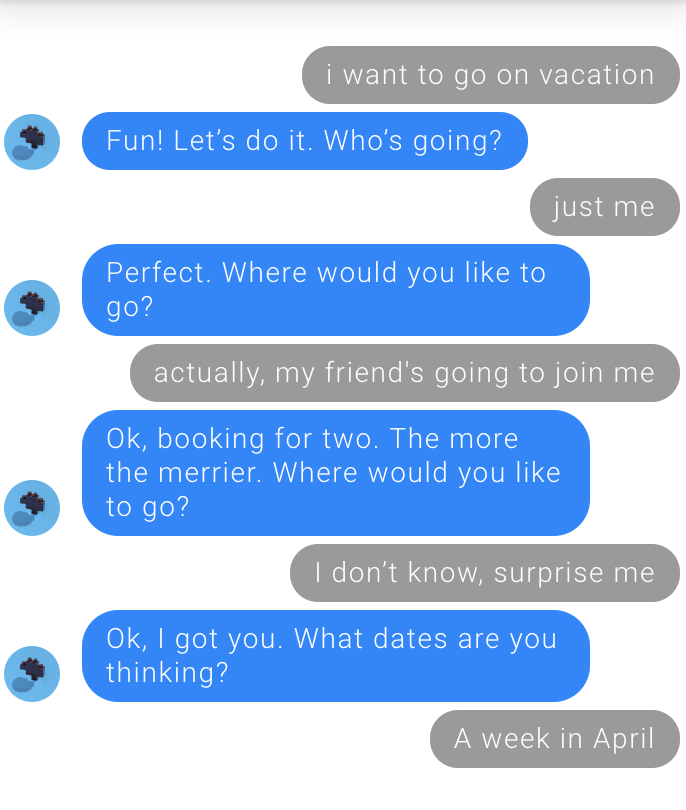
\includegraphics[width=0.3\linewidth,keepaspectratio]{chatbot15}
% \end{center}


% % {\tiny (Ref: The next generation of AI assistants in enterprise -  Alan Nichol)}
% \end{frame}


% %%%%%%%%%%%%%%%%%%%%%%%%%%%%%%%%%%%%%%%%%%%%%%%%%%%%%%%%%%%
% \begin{frame}[fragile]\frametitle{Level 4 : Personalized Assistants}
% \begin{itemize}
% \item the contextual assistant can engage in a flexible back-and-forth with you and offer more than prebuilt answers because it knows how to respond to unexpected user utterances. 
% \item The assistant also begins to understand context at this point. 
% \item For instance, the travel bot will be able to walk you through a few popular destinations and make the necessary travel arrangements.
% \end{itemize}

% \begin{center}
% 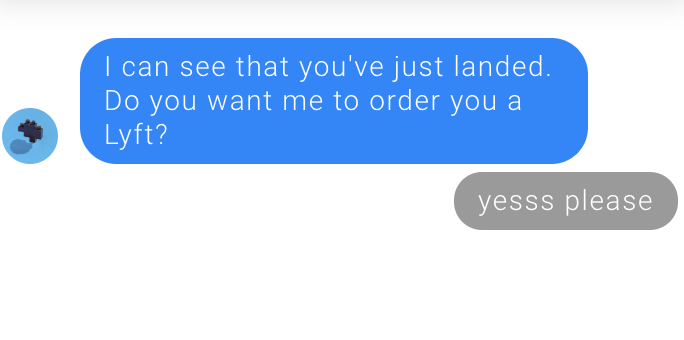
\includegraphics[width=0.6\linewidth,keepaspectratio]{chatbot16}
% \end{center}

% % {\tiny (Ref: The next generation of AI assistants in enterprise -  Alan Nichol)}
% \end{frame}

% %%%%%%%%%%%%%%%%%%%%%%%%%%%%%%%%%%%%%%%%%%%%%%%%%%%%%%%%%%%
% \begin{frame}[fragile]\frametitle{Level 5 and beyond: Autonomous Organization of Assistants}
% \begin{itemize}
% \item contextual assistants are able to monitor and manage a host of other assistants in order to run certain aspects of enterprise operations. 
% \item They'd be able to run promotions on certain travel experiences, target certain customer segments more effectively based on historical trends, increase conversion rates and adoption, and so forth.
% \end{itemize}


% % {\tiny (Ref: The next generation of AI assistants in enterprise -  Alan Nichol)}
% \end{frame}


% %%%%%%%%%%%%%%%%%%%%%%%%%%%%%%%%%%%%%%%%%%%%%%%%%%%%%%%%%%%
% \begin{frame}[fragile]\frametitle{Conversational Chatbot}

% \begin{itemize}
% \item Understands the context of the conversation
% \item Can handle any user goal gracefully
% \item Means that the bot may not be able to answer all questions but it can handle the conversation well.
% \end{itemize}

% Simple conversation:
% \begin{center}
% 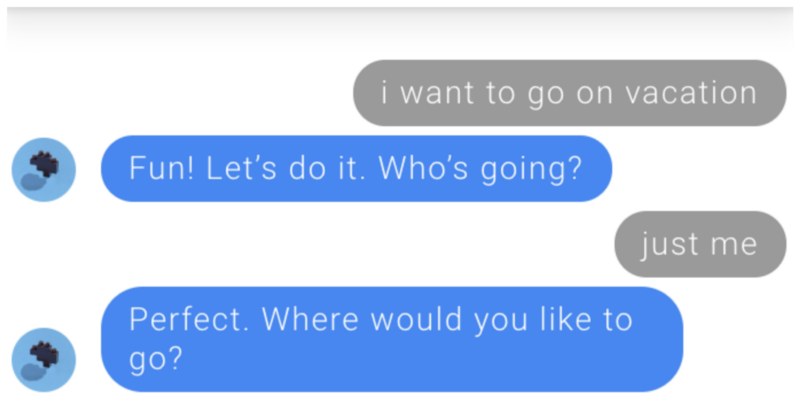
\includegraphics[width=0.6\linewidth,keepaspectratio]{chatbot17}
% \end{center}


% \end{frame}


% %%%%%%%%%%%%%%%%%%%%%%%%%%%%%%%%%%%%%%%%%%%%%%%%%%%%%%%%%%%
% \begin{frame}[fragile]\frametitle{Classification of Chatbots}
% \begin{center}
% 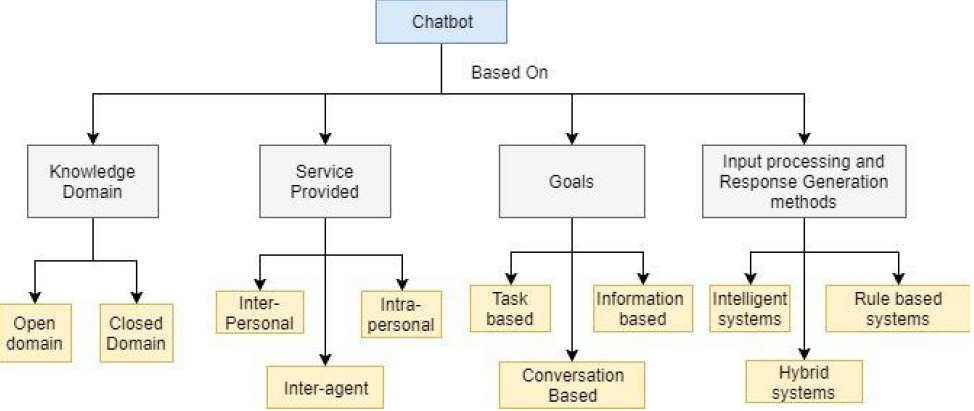
\includegraphics[width=\linewidth,keepaspectratio]{chatbot18}
% \end{center}

% % {\tiny (Ref: Chatbots: An overview. Types, Architecture, Tools and Future Possibilities -  Ketakee Nimavat et al)}
% \end{frame}

% %%%%%%%%%%%%%%%%%%%%%%%%%%%%%%%%%%%%%%%%%%%%%%%%%%%%%%%%%%%
% \begin{frame}[fragile]\frametitle{Why do we need a Chatbot?}

% \begin{itemize}
% \item Chat is the most natural way of interaction between human and application.
% \item Bots are interactive.
% \item Chatbots add a human touch to any application you build.
% \item Bots are engaging. It is not as boring as filling up a long form.
% \end{itemize}

% % {\tiny (Ref: Chatbots 101 - Architecture \& Terminologies -  Bhavani Ravi)}
% \end{frame}


%%%%%%%%%%%%%%%%%%%%%%%%%%%%%%%%%%%%%%%%%%%%%%%%%%%%%%%%%%%
\begin{frame}[fragile]\frametitle{History}

    \begin{columns}
    \begin{column}[t]{0.5\linewidth}
	\begin{itemize}
	\item Chatbot history dates as far back as the 1960s.
	\item Eliza by MIT professor Joseph Weizenbaum: a psychotherapist who responded to the user with questions. Pattern based.
	\item ALICE (``Artificial Linguistic Internet Computer Entity'') chatbot in 1995 by Richard Wallace using AIML (artificial intelligence markup language)
	\item Then of course, most tech giants are at it now \ldots
	\end{itemize}
	
\tiny{(Ref: DUnderstanding AI Chatbots, Challenges, Opportunities \& Beyond - Pramod Chandrayan)}

	
    \end{column}
    \begin{column}[t]{0.5\linewidth}
\begin{center}
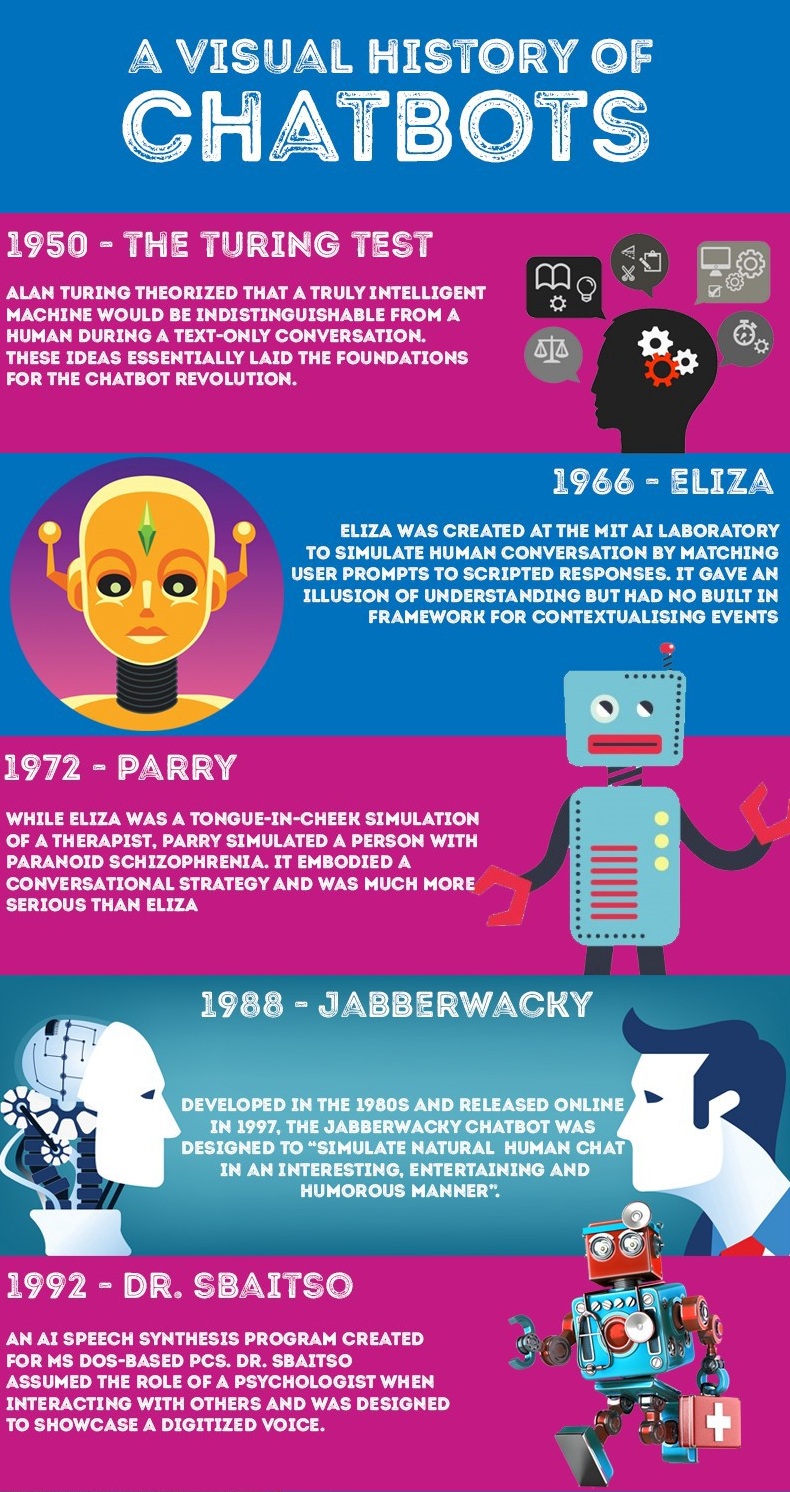
\includegraphics[width=0.6\linewidth,keepaspectratio]{chatbot19a}

\end{center}
    \end{column}
  \end{columns}
  
  

	
\end{frame}

%%%%%%%%%%%%%%%%%%%%%%%%%%%%%%%%%%%%%%%%%%%%%%%%%%%%%%%%%%%
\begin{frame}[fragile]\frametitle{History}

    \begin{columns}
    \begin{column}[t]{0.5\linewidth}
\begin{center}
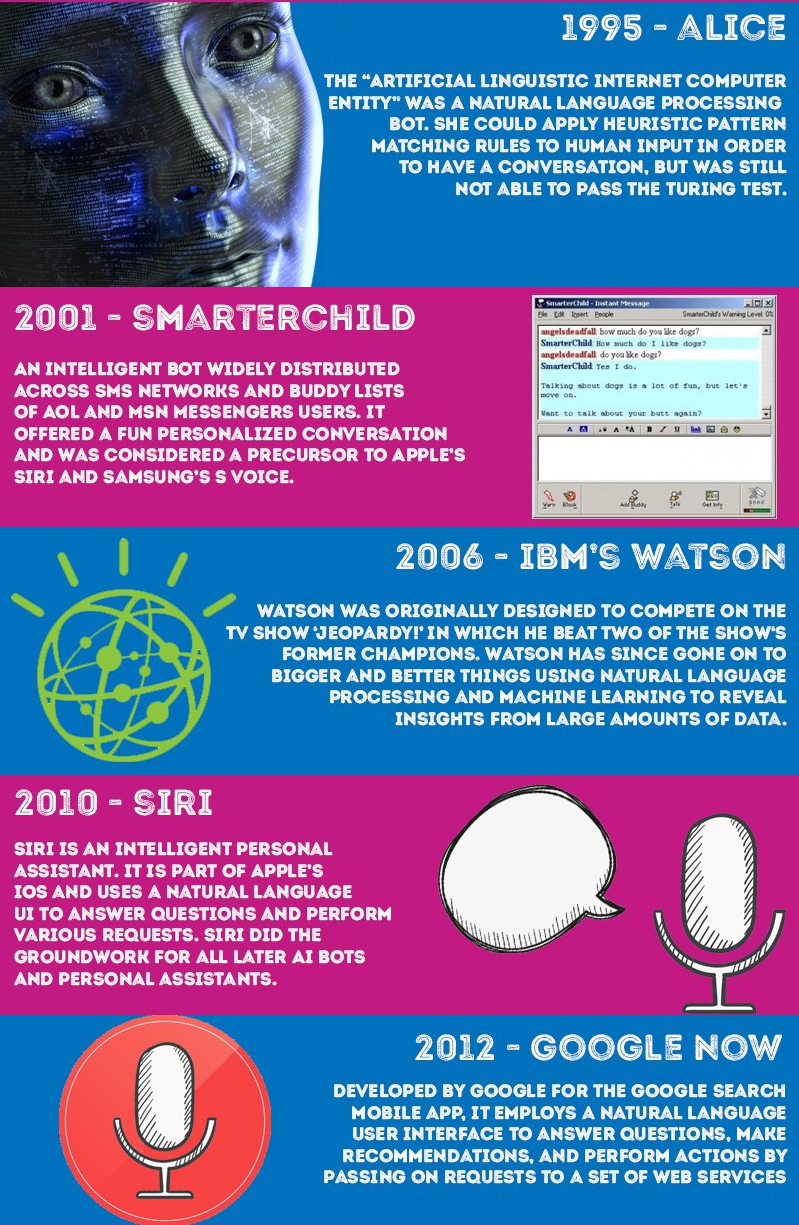
\includegraphics[width=0.6\linewidth,keepaspectratio]{chatbot19b}

\end{center}
    \end{column}
    \begin{column}[t]{0.5\linewidth}
\begin{center}
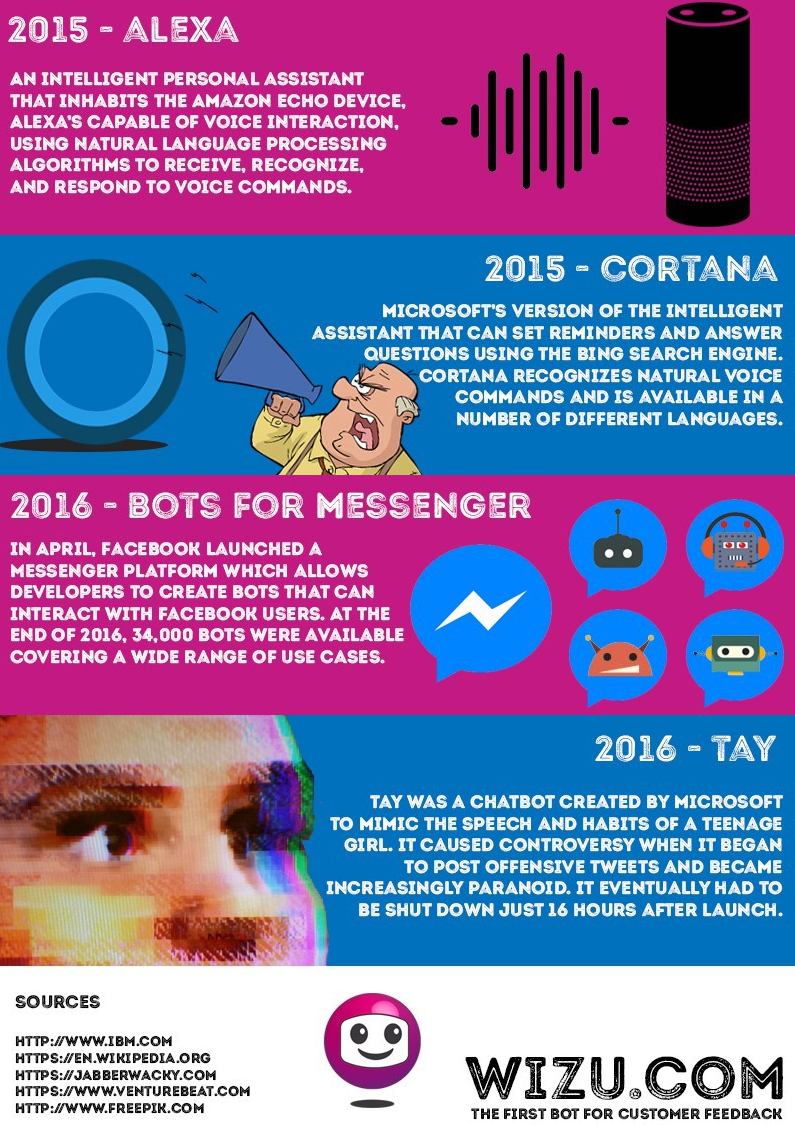
\includegraphics[width=0.6\linewidth,keepaspectratio]{chatbot19c}

\end{center}
    \end{column}
  \end{columns}
  
  

	
\end{frame}


%%%%%%%%%%%%%%%%%%%%%%%%%%%%%%%%%%%%%%%%%%%%%%%%%%%%%%%%%%%
\begin{frame}[fragile]\frametitle{The Giants are at it \ldots}
\begin{center}
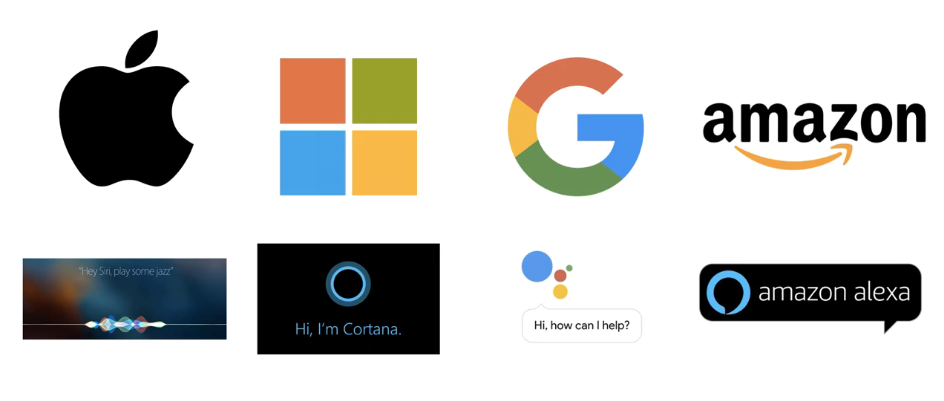
\includegraphics[width=0.8\linewidth,keepaspectratio]{nlp1}

\tiny{(Ref: Deep Learning and NLP A-Z - Kirill Eremenko)}
\end{center}

	\begin{itemize}
	\item Chatbots or QA systems, predominantly voice based, 
	\item Underlying processing is primarily Natural Language Processing (NLP).
	\item You can have your own chatbot, specific to you!! 
	\item NLP is the core skill needed.
	\end{itemize}
	
\end{frame}


%%%%%%%%%%%%%%%%%%%%%%%%%%%%%%%%%%%%%%%%%%%%%%%%%%%%%%%%%%%
\begin{frame}[fragile]\frametitle{Why so much popularity?}
Chatbots are:
	\begin{itemize}
	\item Autonomous and Always Available
	\item Drive Conversation
	\item Able to handle millions of requests, scalable.
	\end{itemize}
	
But to have a good Chatbot, at core, we would need expertize in NLP!!

\end{frame}





% %%%%%%%%%%%%%%%%%%%%%%%%%%%%%%%%%%%%%%%%%%%%%%%%%%%%%%%%%%%
% \begin{frame}[fragile]\frametitle{How are chatbots different from Apps?}

% \begin{itemize}
% \item Chatbots are the most natural way of interaction, it just feels like asking your friend for help but can still do all the activities that a has to do.
% \item Chatbot is like adding a conversational interface to apps.
% \end{itemize}

% {\tiny (Ref: Chatbots 101 - Architecture \& Terminologies -  Bhavani Ravi)}
% \end{frame}

% %%%%%%%%%%%%%%%%%%%%%%%%%%%%%%%%%%%%%%%%%%%%%%%%%%%%%%%%%%%%%%%%%%%%%%%%%%%%%%%%%%
% \begin{frame}[fragile]\frametitle{}
% \begin{center}
% {\Large Forecasts}
% \end{center}
% \end{frame}



%%%%%%%%%%%%%%%%%%%%%%%%%%%%%%%%%%%%%%%%%%%%%%%%%%%%%%%%%%%
\begin{frame}[fragile]\frametitle{Forecasts}

    \begin{columns}
    \begin{column}[t]{0.5\linewidth}
\begin{center}
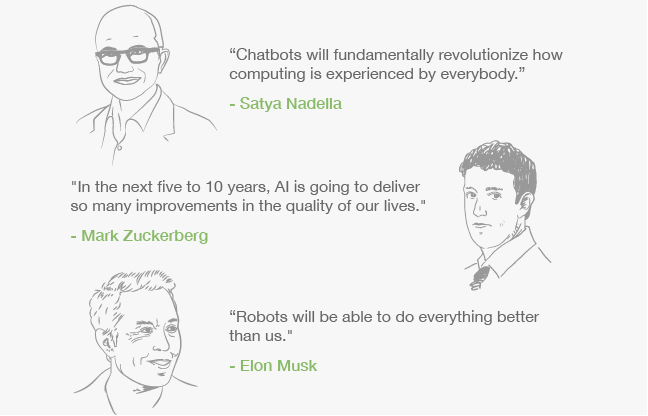
\includegraphics[width=\linewidth,keepaspectratio]{chatbot20a}

\end{center}

\tiny{(Ref: Subro.io)}

    \end{column}
    \begin{column}[t]{0.5\linewidth}
\begin{center}
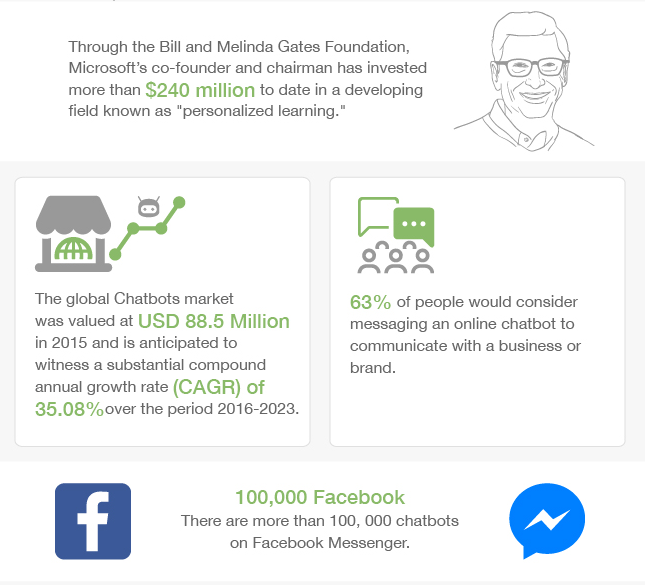
\includegraphics[width=\linewidth,keepaspectratio]{chatbot20b}

\end{center}
    \end{column}
  \end{columns}
  

  
\end{frame}

%%%%%%%%%%%%%%%%%%%%%%%%%%%%%%%%%%%%%%%%%%%%%%%%%%%%%%%%%%%
\begin{frame}[fragile]\frametitle{Forecasts}

    \begin{columns}
    \begin{column}[t]{0.5\linewidth}
\begin{center}
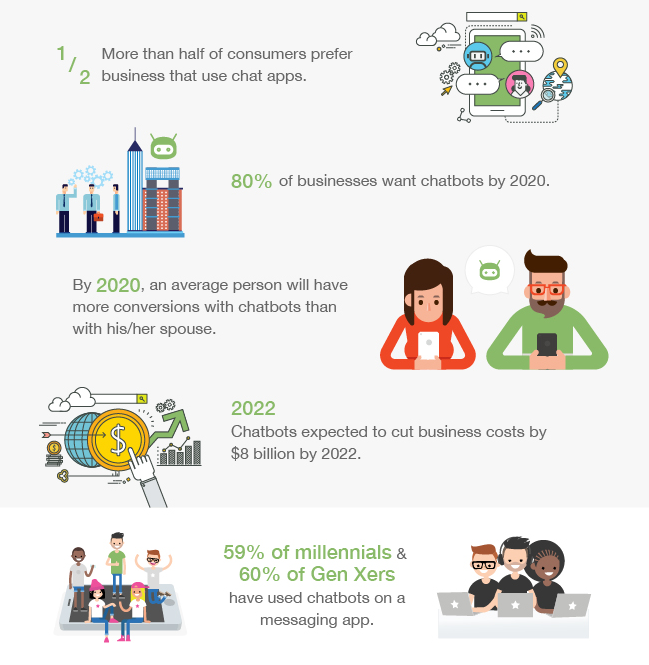
\includegraphics[width=\linewidth,keepaspectratio]{chatbot20c}

\end{center}
    \end{column}
    \begin{column}[t]{0.5\linewidth}
\begin{center}
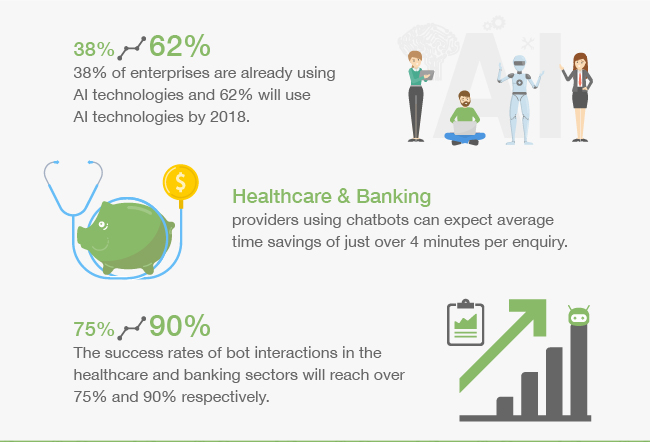
\includegraphics[width=\linewidth,keepaspectratio]{chatbot20d}

\end{center}

\tiny{(Ref: Subro.io)}
    \end{column}
  \end{columns}
  
 
\end{frame}

%%%%%%%%%%%%%%%%%%%%%%%%%%%%%%%%%%%%%%%%%%%%%%%%%%%%%%%%%%%
\begin{frame}[fragile]\frametitle{Challenges for Chatbot}

\begin{itemize}
\item Security:  should ensure that only relevant data is being asked and captured as an input and also is being securely transmitted over the Internet.
\item Making Chatbot stick, like-able and functioning
\item Language Modeling: meaning based vectorization, even for vernacular.
\item etc \ldots
\end{itemize}
\end{frame}

%%%%%%%%%%%%%%%%%%%%%%%%%%%%%%%%%%%%%%%%%%%%%%%%%%%%%%%%%%%
\begin{frame}[fragile]\frametitle{Pros}

	\begin{itemize}
	\item  Anytime, day or night	
	\item Can handle repetitive, boring tasks
	\item Scalable
	\item Consistent
	\item Can gather data
	\end{itemize}


\end{frame}

%%%%%%%%%%%%%%%%%%%%%%%%%%%%%%%%%%%%%%%%%%%%%%%%%%%%%%%%%%%
\begin{frame}[fragile]\frametitle{Cons}

	\begin{itemize}
	\item NLU is hard, AI is not GENERAL yet
	\item Cant design for ANY interaction
	\item Can be Risky
	\item Cant trust for sensitive data
	\end{itemize}


\end{frame}
